\documentclass[professionalfonts,tiny]{beamer}
\setbeamercovered{transparent}
\usepackage{psfig}
%\usetheme{boxes}
%\usecolortheme{beaver}
\usepackage{lipsum}% http://ctan.org/pkg/lipsum
\usepackage{setspace}% http://ctan.org/pkg/setspace
\let\oldframetitle\frametitle% Store old \frametitle in \oldframetitle
\renewcommand{\frametitle}[1]{% Redefine \frametitle
  \oldframetitle{#1}\setstretch{1.25}}
%\setstretch{2} <--- uncomment to see the global effect of \setstretch{2}


\newcommand{\Lower}[1]{\smash{\lower 1.5ex \hbox{#1}}}
\newcommand{\STRUT}{\rule{0in}{3ex}}
\begin{document}

\begin{frame}{Government Budget Constraint}
\footnotesize

\begin{enumerate}
\item Your Credit Card Statement
\item The Government Budget Constraint
\item Expenditure and Revenue Details
\item Deficits and Surpluses
\item The Debt-to-GDP Ratio
\item Stainability
\item Seignorage
\item Iterating Backward and Forward
\end{enumerate}

\end{frame}


\begin{frame}{Your Credit Card Bill}
\footnotesize

\begin{itemize}
\item If you have a credit card, you get a bill each month.
\item Your balance this month is
\begin{eqnarray*}
\mbox{Balance this month}  &=&  \mbox{Balance last month} \\
                && \; + \; \mbox{ Finance Charge} \\
                && \; + \; \mbox{ New Purchases} \\
                && \; - \; \mbox{ Payments}
\end{eqnarray*}
\item Let's re-write this as
\begin{eqnarray*}
B_{t}  &=&  B_{t-1} + r B_{t-1} + G_t - T_t
\end{eqnarray*}
where we let $B$ denote the balance, $r$ denote the monthly interest rate (so $rB$ is the finance charge), $G$ be new purchases, and $T$ be payments.

\end{itemize}

\end{frame}

\begin{frame}{Stock Variables and Flow Variables}

\begin{itemize}

\item {\em Stock variables} are measured at a point in time.

\bigskip

\item {\em Flow variables} are measured over a period of time.

\bigskip

\item So which variables on your credit card balance are stock variables? flow variables?

\end{itemize}

\end{frame}


\begin{frame}{The Government Budget Constraint}
\footnotesize

A sovereign government faces a budget constraint that
must hold at each period, $t$:
\begin{eqnarray*}
B_{t}  &=&  B_{t-1} + r B_{t-1} + G_t + TR_t - T_t
\end{eqnarray*}
where
\begin{eqnarray*}
G_t  &=& \mbox{Government spending during period $t$} \\
TR_t &=& \mbox{Transfer payments (e.g. social security) during period $t$} \\
T_t &=& \mbox{Taxes collected during period $t$} \\
B_{t}  &=& \mbox{This period's ($t$) government debt} \\
r  &=& \mbox{Real interest rate}
\end{eqnarray*}

Many macro textbooks write it this way
\begin{eqnarray*}
B_{t}  &=&  B_{t-1} + INT_t + G_t + TR_t - T_t
\end{eqnarray*}


\end{frame}

\begin{frame}{Fiscal Data: Federal Government}

\begin{itemize}
\item prior to 1790
\begin{itemize}
\item constructed accounts from various reports
\end{itemize}

\bigskip

\item 1790-present
\begin{itemize}
\item U.S. Treasury (1790-1940)
\item Office of Management and Budget (1934-present)
\end{itemize}

\bigskip

\item 1929-present
\begin{itemize}
\item National Income and Product Accounts (NIPA)
\end{itemize}
\end{itemize}

\end{frame}

\begin{frame}{NIPA vs Treasury/OMB}
\footnotesize

NIPA
\begin{itemize}
\item calendar year/quarter, 1929-present
\item consistent accounting with state/local as well as GDP
\item main spending categories
\begin{itemize}
\footnotesize
\item Government consumption, $G_t$
\item Transfer payments, $TR_t$
\item Net interest payments, $INT_t$
\end{itemize}
\end{itemize}
\bigskip
Treasury/OMB
\begin{itemize}
\item fiscal year
\item spending divided by function
\begin{itemize}
\footnotesize
\item pre-1940: war, navy, pensions, indians, interest, ...
\item 1934-present: national defense, human resources, physical resources, net interest, ...
\end{itemize}
\end{itemize}

\end{frame}

\begin{frame}{Comparison Between Federal and State \& Local}

\begin{itemize}

\item Combined U.S. federal, state, and local government together.
\begin{itemize}
\item spending well over 1/3 of GDP.
\end{itemize}

\item Current composition of the  federal government budget is quite different
from state and local budgets.

\item One often hears

\medskip

\begin{quote}
The federal government is a gigantic insurance company with a side business in defense.
\end{quote}

\item State and local governments more directly involved in government purchases

\end{itemize}
\end{frame}

\begin{frame}
\centerline{\psfig{file=all_gov_rec_exp.ps,width=3.8in}}
\vspace{.1in}
\centerline{NIPA: Total Government Receipts and Expenditures as a Percent of GDP}
\end{frame}

\begin{frame}
\centerline{\psfig{file=all_gov_exp_decomp.ps,width=3.8in}}
\vspace{.1in}
\centerline{NIPA: Total Government Expenditures Decomposed By Type}
\end{frame}

\begin{frame}
\centerline{\psfig{file=fed_gov_exp_decomp.ps,width=3.8in}}
\vspace{.1in}
\centerline{NIPA: Federal Expenditures Decomposed By Type}
\end{frame}

\begin{frame}
\centerline{\psfig{file=sl_gov_exp_decomp.ps,width=3.8in}}
\vspace{.1in}
\centerline{NIPA: State and Local Expenditures Decomposed By Type}
\end{frame}

\begin{frame}
\centerline{\psfig{file=fed_expend_decomp_1776_1940.ps,width=3.8in}}
\vspace{.1in}
\centerline{1790-1940: Federal Government Expenditures Decomposed By Type}
\end{frame}

\begin{frame}
\centerline{\psfig{file=federal_expend_decomp_1940_2011.ps,width=3.8in}}
\vspace{.1in}
\centerline{OMB: Federal Government Expenditures Decomposed By Type}
\end{frame}

\begin{frame}
\centerline{\psfig{file=Med_SS_per_GDP.ps,width=3.8in}}
\vspace{.1in}
\centerline{OMB: Medicare and Social Security Spending}
\end{frame}




\begin{frame}{Revenue side}
\footnotesize

NIPA: Six principal categories

\begin{enumerate}
\item Personal taxes:
  \begin{itemize}
\footnotesize
  \item Personal income taxes
  \end{itemize}

 \item Taxes on production and imports
 \begin{itemize}
\footnotesize
 \item sales taxes
 \item property taxes
 \item customs
 \end{itemize}

\item Taxes on corporate income

\item Contributions for Social Insurance
\begin{itemize}
\footnotesize
\item Social Security
\end{itemize}

\item Transfers

\item Other
\begin{itemize}
\footnotesize
\item income on assets and government enterprises
\end{itemize}

       \end{enumerate}
\end{frame}

\begin{frame}
\centerline{\psfig{file=fed_gov_rec_decomp.ps,width=3.8in}}
\vspace{.1in}
\centerline{NIPA: Federal Revenues Decomposed By Type}
\end{frame}

\begin{frame}
\centerline{\psfig{file=sl_gov_rec_decomp.ps,width=3.8in}}
\vspace{.1in}
\centerline{NIPA: State and Local Revenues Decomposed By Type}
\end{frame}

\begin{frame}{Revenue: Federal vs. State/Local}

\begin{itemize}

\item Federal government
\begin{itemize}
\item Income taxes
\item Contributions for social insurance
\end{itemize}

\bigskip

\item State/Local
\begin{itemize}
\item property and sales taxes
\item transfers from the federal government
\end{itemize}

\bigskip

\item Compositional changes for federal government over time
\begin{itemize}
\item customs to internal revenue (income taxes)
\end{itemize}

\end{itemize}

\end{frame}

\begin{frame}
\centerline{\psfig{file=fed_receipts_decomp_1776_1940.ps,width=3.8in}}
\vspace{.1in}
\centerline{1790-1940: Federal Revenues Decomposed By Type}
\end{frame}

\begin{frame}{Deficits and Surpluses}
\footnotesize

\begin{itemize}
\item The budget deficit that gets reported in the newspaper is
$G_t + TR_t + INT_t - T_t$.
\begin{itemize}
\item When this number is positive there is a budget deficit.
\item When this number is negative there is a budget surplus.
\end{itemize}

\item Change in the debt is equal to the deficit
\begin{eqnarray*}
B_{t} - B_{t-1}  =  INT_t + G_t + TR_t - T_t
\end{eqnarray*}

\item The {\em net-of-interest deficit} or {\em primary deficit} is $G_t +
TR_t - T_t$.

\item The total or gross deficit tells the amount the government must borrow to
cover all of its expenditures.

\item The primary deficit ignores interest payments

\end{itemize}

\end{frame}

\begin{frame}
\centerline{\psfig{file=fed_expend_rev_gdp_1775_2011.ps,width=3.8in}}
\vspace{.1in}
\centerline{Federal Government Receipts and Expenditures as Percentage of GDP}
\end{frame}

\begin{frame}
\centerline{\psfig{file=federal_gross_deficit_1770_2011.ps,width=3.8in}}
\vspace{.1in}
\centerline{Federal Government Deficit as a Percentage of GDP}
\end{frame}

\begin{frame}{The Printing Press}
\footnotesize

\begin{itemize}

\item Since the signing of the U.S. Constitution, the Federal government can raise revenue by issuing money.
\begin{itemize}
\footnotesize
\item State and local governments can not.
\end{itemize}

\item For the Federal government
\begin{eqnarray*}
B_{t}  &=&  B_{t-1} + r B_{t-1} + G_t + TR_t - T_t  - \frac{M_t - M_{t-1}}{P_t}
\end{eqnarray*}
where
\begin{eqnarray*}
M_{t}-M_{t-1} &=& \mbox{New money printed this period.} \\
P_t  &=& \mbox{Price level this period ($t$)} \\
     & & \mbox{i.e. the relative price of money in terms of goods}
\end{eqnarray*}

\item This additional term is called {\em seignorage} or the inflation tax.
\end{itemize}

\end{frame}

\begin{frame}

\begin{itemize}

\item So the government budget constraint becomes
\begin{eqnarray*}
B_{t}  &=&  B_{t-1} + r B_{t-1} + G_t + TR_t - T_t  - \frac{M_t - M_{t-1}}{P_t}
\end{eqnarray*}

\item Write it as
\begin{eqnarray*}
B_{t}  -  B_{t-1} + \frac{M_t - M_{t-1}}{P_t}  =  r B_{t-1} + G_t + TR_t - T_t
\end{eqnarray*}

\medskip

\item Decisions about $G_t$, $TR_t$ and $T_t$ are called {\em fiscal
policy}.

\medskip

\item Decision about $B_t$ and $M_t$ are called {\em monetary
policy}.

\end{itemize}

\end{frame}

\begin{frame}{The Debt Limit Debate}
\footnotesize

\begin{itemize}

\item Debt Limit evolved from the funding of the Panama Canal and World War I.

\item Congress sets $G_t$, $TR_t$ and $T_t$, but also says $B_t$ must be less than some number.

\item No big deal up until recently.

\item Congress passes legislation on spending and taxes,
but then many can be reluctant to authorize the debt limit increase
implied by their own spending and tax choices.

\item If not passed either would have to not pay part of $INT$, $G$, or $TR$.

\item True even if $T > INT$.

\end{itemize}

\end{frame}

\begin{frame}{Debt-to-GDP Ratio}
\footnotesize

\begin{itemize}

\item Suppose the credit card balance is \$20,000.  Is this a big balance?

\item Well it depends
\begin{itemize}
\footnotesize
\item If your annual income is \$15,000, then yes.
\item If your annual income is \$1,500,000, then no.
\end{itemize}

\item It also depends on how fast your income is growing.

\item So we might be interested in the ratio of debt-to-income.  Let's call income $Y$, and the ratio of
debt-to-income $\frac{B}{Y}$.

\item What is the current debt-to-GDP ratio?
\end{itemize}

\end{frame}

\begin{frame}
\centerline{\psfig{file=long_total_fed_debt_to_gdp.ps,width=3.8in}}
\vspace{.1in}
\centerline{Federal Debt to GDP Ratio}
\end{frame}

\begin{frame}{A Digression on the U.S. Debt}

\begin{itemize}

\item Marketable Debt
\begin{itemize}
\item Treasury bills, notes, and bonds
\item can be bought and sold on secondary markets
\end{itemize}

\item Non-marketable Debt
\begin{itemize}
\item no secondary market -- saving bonds,  state and local governments
\end{itemize}

\item Held by the Public
\begin{itemize}
\item you, me, China
\end{itemize}

\item Held inside the government
\begin{itemize}
\item Social Security Trust Fund
\end{itemize}

\end{itemize}

\end{frame}

\begin{frame}
\centerline{\psfig{file=different_debt_definitions.ps,width=3.8in}}
\vspace{.1in}
\centerline{U.S. Treasury Debt As A Percent of GDP}
\end{frame}

\begin{frame}{Back to the Government Budget Constraint}

\begin{itemize}

\item Ignore seignorage for now, set $TR = 0$.
\begin{eqnarray*}
B_{t}  &=&  B_{t-1} + r B_{t-1} + G_t - T_t \\
B_{t}  &=&  (1+r) B_{t-1} + G_t - T_t
\end{eqnarray*}

\item Divide both sides of the equation by current income $Y_t$
\begin{eqnarray*}
\frac{B_{t}}{Y_t}  &=&  (1+r) \frac{B_{t-1}}{Y_t} + \frac{G_t - T_t}{Y_t} \\
                   &=&  (1+r) \frac{B_{t-1}}{Y_t}\frac{Y_{t-1}}{Y_{t-1}} + \frac{G_t - T_t}{Y_t} \\
                   &=&  (1+r) \frac{B_{t-1}}{Y_{t-1}}\frac{Y_{t-1}}{Y_{t}} + \frac{G_t - T_t}{Y_t}
\end{eqnarray*}

\end{itemize}

\end{frame}

\begin{frame}

\begin{itemize}

\item Let $g$ denote the percentage change in $Y$
\begin{eqnarray*}
g = \frac{Y_t}{Y_{t-1}} - 1
\end{eqnarray*}
so
\begin{eqnarray*}
\frac{Y_{t-1}}{Y_t} = \frac{1}{1+g}
\end{eqnarray*}

\item So we can write
\begin{eqnarray*}
\frac{B_{t}}{Y_t} &=&  \frac{(1+r)}{(1+g)} \frac{B_{t-1}}{Y_{t-1}} + \frac{G_t - T_t}{Y_t} \\
                  &\approx&  (1+r-g) \frac{B_{t-1}}{Y_{t-1}} + \frac{G_t - T_t}{Y_t} \\
\end{eqnarray*}

\item To keep the math simple, assume $G$ and $T$ are constant over time.

\end{itemize}

\end{frame}

\begin{frame}{Sustainable Fiscal Policy}

\begin{itemize}

\item Most countries have positive debt-to-GDP ratios.

\item In the short-term, it is often no big deal if this ratio rises.

\item But can debt-to-GDP ratios rise forever?
\begin{itemize}
\item debt crisis
\item currency crisis
\item hyperinflation
\end{itemize}

\item In other words, which paths of $B/Y$ are stable? which are explosive?

\end{itemize}

\end{frame}

\begin{frame}

\begin{eqnarray*}
\frac{B_{t}}{Y_t} =  (1+r-g) \frac{B_{t-1}}{Y_{t-1}} + \frac{G - T}{Y_t}
\end{eqnarray*}

\medskip

\begin{itemize}
\item Consider two cases
\begin{enumerate}
\item $g>r$
\item $g \le r$
\end{enumerate}

\medskip

\item If $g > r$, the debt-to-GDP ratio will not blow up.
So a government can sustain persistent deficits as long as growth
in output is greater than the real interest rate.

\medskip

\item In the U.S. $r = 0.016$  and $g = 0.033$.

\medskip

\item Don't necessarily need a balanced budget.

\end{itemize}
\end{frame}

\begin{frame}{Seignorage}

\bigskip

But first, a few basics about money ...


\end{frame}

\begin{frame}{Velocity and the Quantity Theory of Money}

\begin{itemize}

\item Velocity, $V$, measures how much money ``turns over'' each period.
$$ V \equiv {{\mbox{Nominal GDP}}\over{\mbox{nominal money stock}}} =
{{PY}\over{M}}. $$

\item The way the quantity theory of money is usually written is:

\bigskip

\begin{tabular}{ccccccc}
Money & $\times$ & Velocity & = & Price & $\times$ & Output \\
 $M$  & $\times$ & $V$      & = & $P$   & $\times$ &  $Y$  \STRUT \\
\end{tabular}


\item Real money demand is proportional to real income.  So
$${{M^d}\over{P}} = kY $$ Assumes constant velocity.

\end{itemize}

\end{frame}

\begin{frame}{Money and Inflation}

\begin{itemize}

\item Inflation is an increase in the price level. That is, define
inflation as: $$ \pi = \frac{\Delta P}{P} $$

\bigskip

\item A famous quote from Milton Friedman:

\medskip

\begin{quote}
Inflation is always and everywhere a monetary phenomenon.
\end{quote}

\end{itemize}

\end{frame}

\begin{frame}

\begin{itemize}

\item In a world without frictions, doubling the money supply has
no effect on output, it just doubles the price level.  So
$$ \pi = {{P_{t+1} - P_{t}}\over{P_t}} = {{\Delta P}\over{P}} =
{{\Delta M}\over{M}} $$

\item Output does not change, velocity does not change.  Quantity theory
of money.

\medskip

\item Money had no effect on anything anybody cared about.  In other
words money is {\em neutral.}

\medskip

\item The classic dichotomy: money only changes the price level.

\end{itemize}

\end{frame}

\begin{frame}{Deficits and Inflation}

\begin{itemize}

\item Recall the government budget constraint
\begin{eqnarray*}
B_{t}  &=&  B_{t-1} + r B_{t-1} + G_t + TR_t - T_t  - \frac{M_t - M_{t-1}}{P_t}
\end{eqnarray*}

\item Set transfers and government borrowing to zero, so we get
\begin{eqnarray*}
G_t  - T_{t} = {{M_{t} - M_{t-1}}\over{P_t}}
\end{eqnarray*}
So this an all-currency economy.

\item The revenue that a government raises by printing money is called
{\em seignorage}.  This is the inflation tax.

\item Revolutionary War

\end{itemize}

\end{frame}

\begin{frame}{A Great Quote}

\begin{quote}
Lenin is said to have declared that the best way to destroy the
capitalist system was to debauch its currency.  By a continuing
process of inflation, governments can confiscate, secretly and
unobserved, an important wealth of their citizens.
\end{quote}
\smallskip

\noindent{John Maynard Keynes}

\end{frame}

\begin{frame}{Real seignorage and inflation}

\begin{itemize}

\item Consider our all-currency economy. No government debt.

\item If the velocity of money is fixed and output is fixed, so real money demand is constant.
Then $$ \pi = \frac{\Delta P}{P} = \frac{\Delta M}{M} $$

\item Real seignorage revenue, $R$, is
$$ \frac{M_{t} - M_{t-1}}{P_t}  = \frac{\Delta M}{P}.$$
\item Since $\pi = {{\Delta M}\over{M}}$, real seignorage revenue is
$$ R = \pi \frac{M}{P}$$.

\end{itemize}

\end{frame}

\begin{frame}

\begin{itemize}

\item So seignorage is a tax at the rate of inflation on real money balances.
That's why it is called the inflation tax.

\medskip

\item The government collect revenue from the inflation tax when it
buys goods with newly printed money.

\medskip

\item So Friedman's really should have said,
\begin{quote}
Inflation is always and everywhere a fiscal phenomenon.
\end{quote}

\medskip

\item Since seignorage is a distortionary tax, as the government
increases this tax, people will hold lower real balances.

\medskip

\item Whether seignorage rises or falls depends on whether inflation
rises more or less than the decline in money holdings.

\end{itemize}

\end{frame}

\begin{frame}{Government Debt is a Weighted Accumulation of Past Deficits}

\begin{itemize}

\item To keep the analysis simple, ignore transfers and money creation for now.

\item A time $t$ the G.B.C. is:
\begin{eqnarray*}
B_{t}  &=&  (1+r)B_{t-1} + G_t  - T_t
\end{eqnarray*}

\item A time $t-1$ the G.B.C. is:
\begin{eqnarray*}
B_{t-1}  &=&  (1+r)B_{t-2} + G_{t-1}  - T_{t-1}
\end{eqnarray*}

\item A time $t-2$ the G.B.C. is:
\begin{eqnarray*}
B_{t-2}  &=&  (1+r)B_{t-3} + G_{t-2}  - T_{t-2}
\end{eqnarray*}

\end{itemize}

\end{frame}

\begin{frame}

\begin{itemize}


\item Substitute for $B_{t-1}$
\begin{eqnarray*}
B_{t}  &=&  (1+r) \left((1+r)B_{t-2} + G_{t-1}  - T_{t-1} \right)  + G_t  - T_t \\
       &=&  (1+r)^2 B_{t-2} +(1+r)\left( G_{t-1}  - T_{t-1} \right)  + G_t  - T_t
\end{eqnarray*}
\item Substitute for $B_{t-2}$
\begin{eqnarray*}
B_{t}  &=&  (1+r)^3 B_{t-3} + (1+r)^2\left( G_{t-2}  - T_{t-2} \right) \\
       & & + (1+r)\left( G_{t-1} - T_{t-1} \right)  + G_t  - T_t
\end{eqnarray*}

\item Keep going to the beginning of time (i.e. $t=0$)
\begin{eqnarray*}
B_{t}  &=&  (1+r)^t B_{0} + \sum_{j=0}^{t} (1+r)^j \left( G_{t-j}  - T_{t-j} \right)
\end{eqnarray*}

\end{itemize}

\end{frame}

\begin{frame}{Government Debt is a Weighted Sum of Future Surpluses}

\begin{itemize}

\item A time $t$ the G.B.C. is:
\begin{eqnarray*}
B_{t}  &=&  (1+r)B_{t-1} + G_t  - T_t
\end{eqnarray*}

\item A time $t+1$
\begin{eqnarray*}
B_{t+1}  &=&  (1+r)B_{t} + G_{t+1}  - T_{t+1}
\end{eqnarray*}
or
\begin{eqnarray*}
B_{t}  &=&  \frac{1}{1+r} \left( B_{t+1} + T_{t+1}  - G_{t+1} \right)
\end{eqnarray*}

\end{itemize}

\end{frame}

\begin{frame}

\begin{itemize}

\item Thus we can write $B_{t+1}$ as
\begin{eqnarray*}
B_{t+1}  &=&  \frac{1}{1+r} \left( B_{t+2} + T_{t+2}  - G_{t+2} \right)
\end{eqnarray*}

\item Substitute
\begin{eqnarray*}
B_{t}  &=&  \frac{1}{1+r} \left( \frac{1}{1+r}\left( B_{t+2} + T_{t+2}  - G_{t+2} \right)+ T_{t+1}  - G_{t+1} \right)
\end{eqnarray*}

\item Do this 100 times
\begin{eqnarray*}
B_{t}  &=&  \left(\frac{1}{1+r}\right)^{100} B_{t+100}  + \sum_{j=1}^{100} \left(\frac{1}{1+r}\right)^{j}(T_{t+j} -G_{t+j})
\end{eqnarray*}

\item Do this an infinite number of times
\begin{eqnarray*}
B_{t}  &=&   \sum_{j=1}^{\infty} \left(\frac{1}{1+r}\right)^{j}(T_{t+j} -G_{t+j})
\end{eqnarray*}

\end{itemize}

\end{frame}

\begin{frame}{Debt is both a backward-looking and a forward-looking variable}

\begin{itemize}

\item Sum of past spending

\bigskip

\item Sum of future surpluses

\end{itemize}
\bigskip

\bigskip
\footnotesize{just like your credit card balance ...}


\end{frame}

\end{document}
